\section{Model predictive control}\label{se:model_predictive_control}
In this section, the design of the controller is elaborated. First the control problem the design of the Model predictive controller (MPC). 

The simulation covered in chapter \ref{ch:simulation} is to be controlled with respect to the problems elaborated in section \ref{sec:problem_statement} and stated here. 
\begin{enumerate}
\item Flow variations due to large industries and natural phenomenons
\item Concentration variations due to large industries and natural phenomenons
\begin{enumerate}
	\item Chloride variations
	\item Phosphor variations
	\item Nitrogen variations
	\item Organic matter variations
\end{enumerate}
\end{enumerate}

From the problem statement, it is stated that flow and concentration variations must be kept to a minimum without causing any overflow in the sewer. To achieve this, tanks are used, these are placed in the sewer network to find locations where they are able to hold back disturbance that will otherwise cause flow and concentration variations into the WWTP. However, the output of these tanks must be controlled in a way where overflow in the tank is prohibited. Therefore the controller must control the output of these tanks in an optimal manner to keep the input variations to the WWTP at a minimum and still be controlled according to some constraints.

To obtain such an optimal behavior MPC is chosen as stated in section \ref{sec:problem_statement}. MPC solves a optimizations problem at each time instant, k, where the main point is to compute a control vector, u that is feed to the system. 

%is an advanced control method which depends on a dynamic model of the system. Where the model, constraints and a cost function is used to generate the most optimal sequence of control inputs to the system, thus obtaining a desired process behavior. However, only the first control input is used in the current timeslot. Hereafter, in the next timeslot, the MPC algorithm is recalculated to find the must optimal input signal for this timeslot and so on. In addition, MPC also take future disturbance into account thereby predicting an output sequence that is optimal including the disturbance. 
An MPC algorithm consists of:
\\ 
\textbf{Cost function} or control objective,$\CMcal{J}$, is an algorithm measuring e.g. the difference between future outputs and a reference while at the same time instant recognizing that any control action is costly for the system. Therefore the price is measured in the cost function over the prediction horizon, $H_p$. This function is therefore minimized with the respect to the future control vector to keep the cost minimized. Furthermore, only the first control input from the vector is used in each time instant thus this optimization is process is calculated at each time step where a new control input is calculated \cite{mpc_control_lecture_notes}.

\textbf{Constraints} is unique advantages of MPC. Constraints can be applied to the process variables e.g. constraints can be set on the states of the system not allowing them to go below a certain value or above. Constraints are usually written as inequality constraint $Ax(k)\leq b$ where the constraint a subject to the optimization problem \cite{mpc_control_lecture_notes}.   

\textbf{Prediction model} for the MPC to be able to predict future system behavior it needs a model to predict from. The model describes the input output behavior of the system. The model will mainly be used to predict the output of the system over the prediction horizon \cite{mpc_control_lecture_notes}.  
%The main advantage of MPC  Furthermore, MPC can be used with constraints to calculate the most optimal control output at the given timeslot and taking disturbance into the account. 
% In figure \ref{fig:control_of_sewer} it is shown that the MPC controller is setting the input to the pump.

% \begin{figure}[H]
% \centering
% 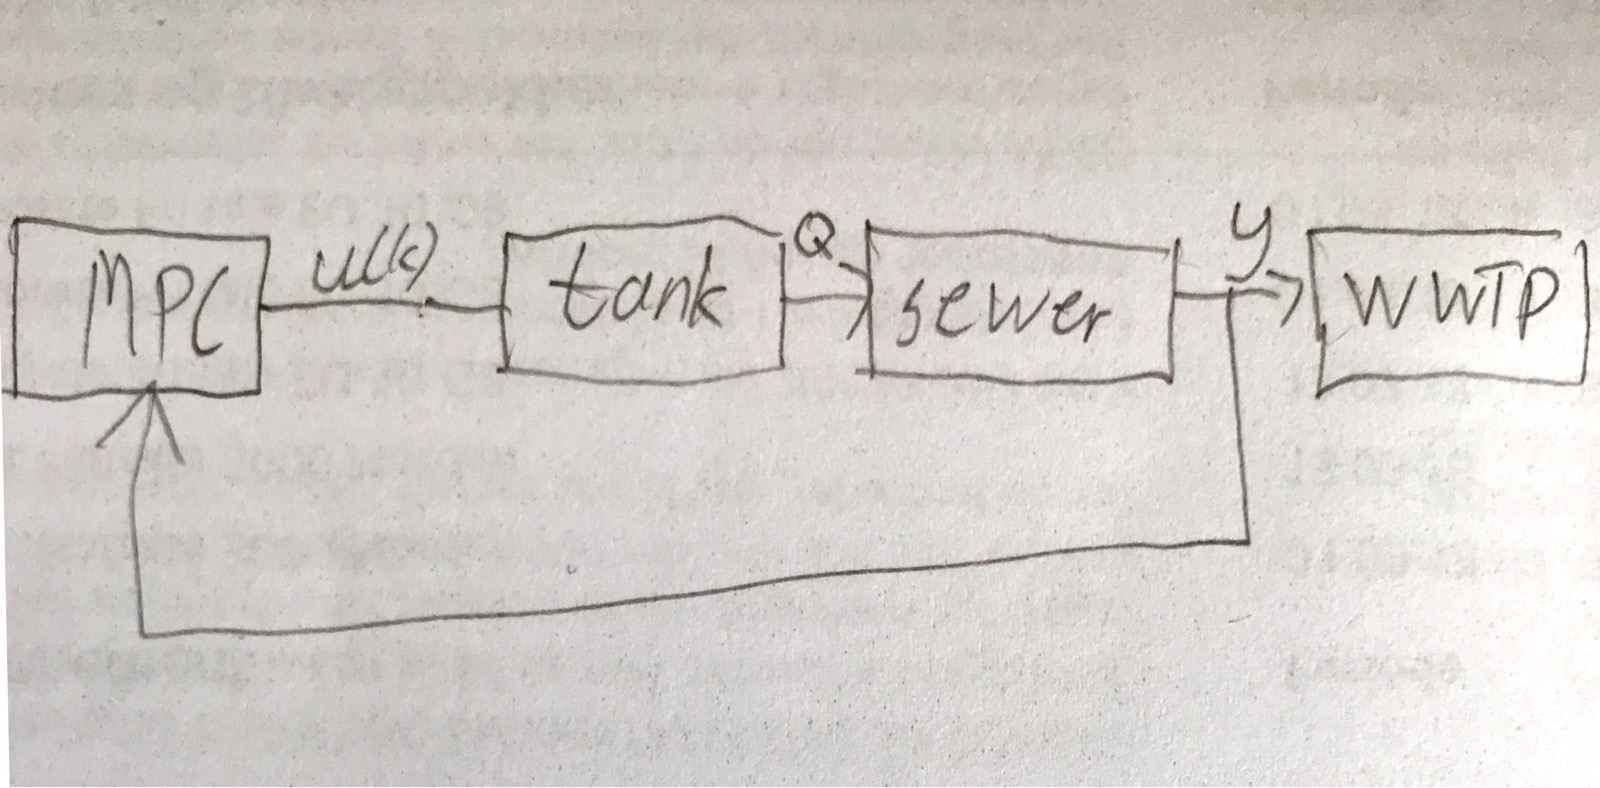
\includegraphics[width=0.8\textwidth]{report/control/pictures/control_of_sewer.jpg}
% \caption{Block diagram of the system.}
% \label{fig:control_of_sewer}
% \end{figure}\fxnote{Der skal staa pumpe i stedet for tank}

% Where the iteration the in the MPC block can be described with the following items. 
% \begin{enumerate}
%        	\item Measurement is taken on the output if possible or it is taken directly from the states. If a state measurement is not available the state is estimated.
%        	\item Calculates a optimal set of predicted values over the prediction horizon according to a cost function and the constraints.
%        	\item The first element of the calculated control sequence is used as the control input.
%        	\item Repeat from 1.
% \end{enumerate}       

For MPC to optimize the system a cost function must be written to penalize variations of the flow output $Q(k+i|k)$ and the concentration output $C(k+i|k)$. Where k defines the time step and i is a value going from $1\leq H_p$. The cost function for flow and concentration is:

\begin{equation}
	 \CMcal{J} = \sum_{i=1}^{H_p-1} || Q(k+i|k)C(k+i|k)-Q(k+i-1|k)C(k+i-1|k)||_{\CMcal{Q}(i)}^2
\end{equation}
Where J is the cost function that needs to be minimized, Q is the flow, C is the concentration and $\CMcal{Q}$ is a weighting parameter. It has been desired to only look at flow variation in the simulation and thereby excluding concentration from the cost function. This has been done to limit the control problem and ease the computation to begin with. Thereby the cost function has been rewritten to: 

\begin{equation}\label{eq:cost_function_height}
	 \CMcal{J} = \sum_{i=1}^{H_p-1} || \hat{y}(k+i|k)-\hat{y}(k+i-1|k)||_{\CMcal{Q}(i)}^2
\end{equation}
\begin{equation}
	\begin{aligned}
	\text{s.t.} \hspace{5mm}  \hat{x}(k+i+1) &= A\hat{x}(k+i|k)+B\hat{u}(k+i|k)+B_dd(k+i|k) \\
						      \hat{y}(k+i)&= C\hat{x}(k+i|k) \\
						     \underline{x} \leq \hat{x} \leq \overline{x}
	\end{aligned}
\end{equation}
Where Q has been replaced with the output y as it can be measured directly from the state space system. The hat denotes a small signal value, and not an estimate for y. y corresponds to the height of the wastewater in the channel, however, it is the same to minimize height difference as the flow because both describe the variation in the output of the sewer. Furthermore, the cost function is subject to constraints for the states. The states have a lower and upper constraint corresponding respectively to the bottom of the channel and the top of the channel, denoted respectively with $\underline{x}$ and $\overline{x}$. In order for the controller to minimize the variations in the output, it must be able to predict future events from knowing the current state. Therefore, by iterating the linear model up to the prediction horizon the controller is able to predict future states \cite{maciejowski2002predictive}. Thus by using the state equation recursively the state equation can be predicted up to the prediction horizon as shown in equation \ref{eq:iterating_state_equation}: 

\begin{equation}\label{eq:iterating_state_equation}
\begin{aligned}
	\hat{x}(k+1|k) &= A\hat{x}(k|k)+B\hat{u}(k|k) + B_dd(k|k)\\
	\hat{x}(k+2|k) &= A\hat{x}(k+1|k)+B\hat{u}(k+1|k)+ B_dd(k+1|k) \\
				   &= A^2\hat{x}(k|k)+AB\hat{u}(k|k)+AB_dd(k|k) + B\hat{u}(k+1|k) \\
				   &+ B_dd(k+1|k) \\
				   &\hspace{2mm}\vdots\\
   \hat{x}(k+H_p|k)&= A\hat{x}(k+H_p-1|k)+B\hat{u}(k+H_p-1|k)+B_dd(k+H_p-1|k)\\
   				   &= A^{H_p}\hat{x}(k|k)+A^{H_p-1}B\hat{u}(k|k)+A^{H_p-1}B_dd(k|k)+\cdots+\\
   				   &+B\hat{u}(k+H_p-1|k)+B_dd(k+H_p-1|k)
\end{aligned}
\end{equation}
Here the first equation $\hat{x}(k+1|k)$ is inserted into the second and this is iterated up to the prediction horizon. This can be setup as prediction vectors and matrices denoted by $\CMcal{X,A,B,U,B}_d$ and $\CMcal{D}$:


\begin{equation}\label{eq:lifted_state_equation}
\begin{aligned}
	  \underbrace{\begin{bmatrix}
	  \hat{x}(k+1|k) 	\\
	  \hat{x}(k+2|k) 	\\
	  \vdots 			\\
	  \hat{x}(k+H_p|k) 	\\
	   \end{bmatrix}}_{\CMcal{X}}
	 &=
	\underbrace{\begin{bmatrix}
		A \\
		A^2 \\
		\vdots \\
		A^{H_p} \\
	\end{bmatrix}}_{\CMcal{A}}
	\hat{x}(k|k) \\&+
	\underbrace{\begin{bmatrix}
		B 		 &0			 &\cdots	& 0		\\
		AB  	 &B  		 & \cdots& 0		\\
		\vdots 	 &\vdots	 & \ddots&\vdots	\\
		A^{H_p-1}B&A^{H_p-2}B&\cdots &B 
    \end{bmatrix}}_{\CMcal{B}}
    	\underbrace{\begin{bmatrix}
	\hat{u}(k|k)\\
	\hat{u}(k+1|k)\\
	\vdots\\
	\hat{u}(k+H_p-1|k)
	\end{bmatrix}}_{\CMcal{U}} \\ &+ 
    \underbrace{\begin{bmatrix}
    	B_d 	    &0	         &\cdots & 0		\\
		AB_d  	    &B_d  	     & \cdots& 0		\\
		\vdots 	    &\vdots	     & \ddots&\vdots	\\
		A^{H_p-1}B_d&A^{H_p-2}B_d&\cdots &B_d 
 %   	B & \cdots & 0 \\
 %    	AB+B & \cdots & 0 \\
 %    	\vdots & \ddots & \vdots \\
 %    	\sum_{i=0}^{H_u-1}A^i B & \cdots & B \\
 %    	\sum_{i=0}^{H_u}A^i B & \cdots & AB+B\\
 %    	\vdots & \vdots & \vdots \\
 %    	\sum_{i=0}^{H_p-1}A^i B & \cdots & \sum_{i=0}^{H_p-H_u}A^i B \\
	  \end{bmatrix}}_{\CMcal{B}_d} 
	\underbrace{\begin{bmatrix}
	d(k|k)\\
	d(k+1|k)\\
	\vdots\\
	d(k+H_p-1|k)
	\end{bmatrix}}_{\CMcal{D}}
	\end{aligned}
\end{equation}

Where $\CMcal{X}$ is the predicted state vector for the entire prediction horizon. $\CMcal{A}$ is the state matrix up to the prediction horizon. $x(k|k)$ is the initial state and is used to predict the hole prediction horizon, $\CMcal{B}$ is the input matrix for the prediction horizon, $\CMcal{U}$ is the predicted input vector, which consists of all the predicted inputs from the current timestep until $(k+H_p-1)$. $\CMcal{B}_d$ is the disturbance matrix for the prediction horizon and $\CMcal{D}$ is the disturbance vector. 

This iteration process is also done for the output equation:

\begin{equation}\label{eq:lifted_output_equation}
	\CMcal{Y}(k)= 
	\begin{bmatrix}
	y(k+1|k)\\
	y(k+2|k)\\
	\vdots\\
	y(k+H_p-1|k)
	\end{bmatrix}
	= 
	\underbrace{\begin{bmatrix}
	C 		& 0 	&\cdots	& 0\\
	0 		& C 	&\cdots & 0 \\
	\vdots	& \vdots&\ddots & 0\\
	0 		& 0		&0 		& C
	\end{bmatrix}}_{\CMcal{C}}
	  \begin{bmatrix}
	  \hat{x}(k+1|k) 	\\
	  \hat{x}(k+2|k) 	\\
	  \vdots 			\\
	  \hat{x}(k+H_p|k) 	\\
	   \end{bmatrix}
\end{equation}
Where $\CMcal{C}$ is a diagonal matrix with the output matrix C and $\CMcal{X}$ the predicted state vector. By inserting the predicted state equation \ref{eq:lifted_state_equation}, into the predicted output equation \ref{eq:lifted_output_equation} the following is achieved:

\begin{equation}\label{eq:output_eq_with_state_eq}
	\CMcal{Y}(k) =  \CMcal{C}\CMcal{A}x(k) +  \CMcal{C}\CMcal{B}\CMcal{U}(k) +\CMcal{C}\CMcal{B}_d\CMcal{D}(k)
\end{equation}   

By using the following notation on equation \ref{eq:output_eq_with_state_eq}:


\begin{equation}
 \psi = \CMcal{C}\CMcal{A}  \hspace{5mm} \gamma = \CMcal{C}\CMcal{B} \hspace{5mm}  \Theta = \CMcal{C}\CMcal{B}_{d}
\end{equation}

The predicted output equation can be rewritten as: 

\begin{equation}\label{eq:lifted_output_with_states_inserted}
	\CMcal{Y}(k) = \psi x(k) + \gamma \CMcal{U}(k) + \Theta \CMcal{D}(k)
\end{equation}

To be able to use the cost function, equation \ref{eq:cost_function_height}, it has to be rewritten so the predicted output equation can be used. This is done by replacing the output y with the predicted output $\CMcal{Y}$ thereby the following is obtained:

\begin{equation}
	\CMcal{J} = ||\CMcal{Y}(k)-\CMcal{Y}(k-1)||_{\CMcal{Q}(i)}^2
\end{equation}
Where the difference between $\CMcal{Y}(k)$ and $\CMcal{Y}(k-1)$ can be expressed as:

\begin{equation}
	\Delta \CMcal{Y}(k) =\CMcal{Y}(k)-\CMcal{Y}(k-1) 
\end{equation}

Thereby the following cost function is achieved:

\begin{equation}\label{eq:delta_cost_function}
	J = \Delta\CMcal{Y}(k)^T \cdot Q \cdot \Delta\CMcal{Y}(k)
\end{equation}

To be able to write the cost function as quadric and linear terms of the predicted output $\Delta\CMcal{U}$, equation \ref{eq:lifted_output_with_states_inserted} is therefore inserted into equation \ref{eq:delta_cost_function} and thereby the following is obtained:

\begin{equation}\label{eq:cost_function_with_all_the_crap}
	\CMcal{J} = (\psi\Delta x(k) + \gamma\Delta \CMcal{U}(k) + \Theta\Delta \CMcal{D}(k))^T\cdot Q \cdot (\psi\Delta x(k) + \gamma\Delta \CMcal{U}(k) + \Theta\Delta \CMcal{D}(k))
\end{equation}

The term on the right hand side of equation \ref{eq:cost_function_with_all_the_crap} is equal to:

\begin{equation}\label{eq:cost_function_big_eq}
	\begin{aligned}
	&(\psi\Delta x(k) + \gamma\Delta \CMcal{U}(k) + \Theta\Delta \CMcal{D}(k))^T\cdot Q \cdot (\psi\Delta x(k) + \gamma\Delta \CMcal{U}(k) + \Theta\Delta \CMcal{D}(k)) = \\
	& \Delta x(k)^T\psi ^T Q \psi \Delta x(k) 								+ \underbrace{\Delta x(k)^T \psi ^T Q \gamma \Delta  \CMcal{U}(k) }_{Linear}				+\Delta x(k)^T \psi ^T Q \Theta \Delta \CMcal{D}(k) \\
	& \underbrace{\Delta \CMcal{U}(k)^T \gamma ^T Q \psi\Delta x(k)}_{Linear} + \underbrace{\Delta \CMcal{U}(k)^T\gamma ^T Q \gamma\Delta \CMcal{U}(k)}_{Quadric} +\underbrace{\Delta \CMcal{U}(k)^T \gamma ^T Q\Theta \Delta \CMcal{D}(k)}_{Linear} \\ 
	& \Delta \CMcal{D}(k)^T \Theta ^T Q  \psi \Delta x(k)					+ \underbrace{\Delta \CMcal{D}(k)^T \Theta ^T Q \gamma  \Delta \CMcal{U}(k) }_{Linear}	+\Delta \CMcal{D}(k)^T \Theta ^T Q \Theta \Delta \CMcal{D}(k)
	\end{aligned}
\end{equation}

Here the quadric and linear terms of $\Delta \CMcal{U}$ are denoted respectively, the remaining terms are the constants and these are not denoted in the equation, however, they will be referred to in the following equations as, c. The quadric variables are collected in: 

\begin{equation}
	\CMcal{H} = \gamma^T Q\gamma 
\end{equation}

And the linear variables are collected in:
\begin{equation}
	\begin{aligned}
	\CMcal{G} &= 2 \Delta x(k)^T\psi^T Q \gamma+2 \Delta \CMcal{D}(k)^T\Theta^T Q \gamma 
	\end{aligned}
\end{equation}

Thereby inserting these expressions in equation \ref{eq:cost_function_big_eq} the final cost function is obtained:

\begin{equation}\label{eq:the_cost_function}
	\min_{\Delta \CMcal{U}(k)} \CMcal{J}(\Delta \CMcal{U}(k)) =\min_{\Delta \CMcal{U}(k)} \Delta \CMcal{U}(k)^T\CMcal{H}\Delta \CMcal{U}(k)+\CMcal{G}\Delta \CMcal{U}(k)+c
\end{equation}

\textbf{Constraints}

In order to apply the constraints, shown in equation \ref{eq:cost_function_height} for the states, to the optimization problem in equation \ref{eq:the_cost_function} the constraints must be reformulated so they are a constraint of the controller input $\Delta\CMcal{U}$, therefore it is required to reformulate the inequalities constraints. 

The constraints applied to the states are upper and lower bound to the channel and the tank, thereby not allowing the simulation to overfill the channel or the tank, or, to have negative height in either of the two. In the following equation the constraint for the states is shown:  


\begin{equation}
	\underline{x} \leq \hat{x} \leq \overline{x}
\end{equation}

As the $\hat{x}$ is a small signal value and as the constraint is for full signal values the operating point needs to be subtracted from the lower and upper bounds thereby transforming the lower and upper bound to small signals:

\begin{equation}
	\underline{x}- \bar{x} \leq \hat{x} \leq \overline{x}-\bar{x}
\end{equation}

To reformulated the constraint the predicted state equation \ref{eq:lifted_state_equation} is inserted instead of the state vector.

\begin{equation}
 	\underline{x}- \bar{x} \leq \CMcal{A}\hat{x}+\CMcal{B}\CMcal{U}+\CMcal{BD} \leq \overline{x}-\bar{x}
 \end{equation} 



\begin{equation}
 	\underline{x}- \bar{x} \leq \CMcal{A}\Delta\hat{x}+\CMcal{B}\Delta\CMcal{U}+\CMcal{B}\Delta\CMcal{D} \leq \overline{x}-\bar{x}
 \end{equation} 


 Now the constraint are setup as constraint on the input signal. In addition, this constraint has to be as equality constraints therefore it is divided into two constraints. 

 \begin{equation}
   	\underbrace{\underline{x}- \bar{x}-\CMcal{A}\Delta\hat{x}-\CMcal{B}\Delta\CMcal{D}}_{x_1}\  \leq \CMcal{B}\Delta\CMcal{U}
 \end{equation}  

 \begin{equation}
 	\underbrace{\overline{x}-\bar{x}-\CMcal{A}\Delta\hat{x}-\CMcal{B}\Delta\CMcal{D}}_{x_2}\geq \CMcal{B}\Delta\CMcal{U}
 \end{equation}


 \begin{equation}
    	\begin{bmatrix}
	   	\CMcal{B}\\
	   	-\CMcal{B}
	   	\end{bmatrix}
	   	\Delta\CMcal{U}
	   	\leq 
	   	\begin{bmatrix}
 		x_1\\
 		x_2
	   	\end{bmatrix}
 \end{equation}

